\documentclass[a4paper]{article}
\usepackage[utf8]{inputenc}
\usepackage[T1]{fontenc}
\usepackage[pdftex]{graphicx}
\usepackage{fancyhdr}
\usepackage{lscape}
\usepackage{color}
\usepackage{qtree}
\usepackage[english]{babel}
\usepackage{graphicx}
\usepackage[colorinlistoftodos]{todonotes}
\usepackage{listings}
\usepackage{color}
\usepackage{float}
\usepackage{changepage}
\usepackage[margin=1in]{geometry}
\definecolor{codegreen}{rgb}{0,0.6,0}
\definecolor{codegray}{rgb}{0.5,0.5,0.5}
\definecolor{codepurple}{rgb}{0.58,0,0.82}
\definecolor{backcolour}{rgb}{0.95,0.95,0.92}
\usepackage[parfill]{parskip}
 \usepackage{ragged2e}
 \lstdefinestyle{mystyle}{
 	backgroundcolor=\color{backcolour},   
 	commentstyle=\color{codegreen},
 	keywordstyle=\color{magenta},
 	numberstyle=\tiny\color{codegray},
 	stringstyle=\color{codepurple},
 	basicstyle=\footnotesize,
 	breakatwhitespace=false,         
 	breaklines=true,                 
 	captionpos=b,                    
 	keepspaces=true,                 
 	numbers=left,                    
 	numbersep=5pt,                  
 	showspaces=false,                
 	showstringspaces=false,
 	showtabs=false,                  
 	tabsize=2
 }
 
\lstset{
	style=mystyle,
	inputencoding=utf8,
	extendedchars=true,
	literate={á}{{\'a}}1 {ã}{{\~a}}1 {é}{{\'e}}1,
	escapechar=\&
}
\title{Algorithmique et structures de données : Mission 6}
\date{1 décembre 2014}
\author{Groupe 1.2: Ivan Ahad - Jérôme Bertaux - Rodolphe Cambier \\ 
	Baptiste Degryse - Wojciech Grynczel - Charles Jaquet}



\begin{document}
\maketitle
\paragraph{Question 1 (Baptiste Degryse)   Un graphe G comportant n noeuds et m arêtes est représenté par la structure Edge List
et les conteneurs V et E sont supposés implémentés par des listes doublement chaînées. Justifiez pourquoi la complexité temporelle de la méthode removeVertex est en O(m) alors que les complexités des méthodes remove-Edge et insertVertex sont en O(1)? Votre réponse à cette question dépend-
elle de la structure de données utilisées pour mémoriser les conteneurs
V et E? En quoi le concept de
location-aware entry
est-il important pour justifier certaines
de ces complexités ?}
Le graphe étant stocké dans une structure Edge List, il faut retrouver le Vertex dans une liste d'edges, en vérifiant à chaque fois si l'edge ne contient pas un pointer vers le vertex, si oui, il faut retirer l'edge. C'est une opération de complexité temporelle O(m) parce qu'il faut toujours tout vérifier pour ne pas rater d'edge.\\
\begin{center}
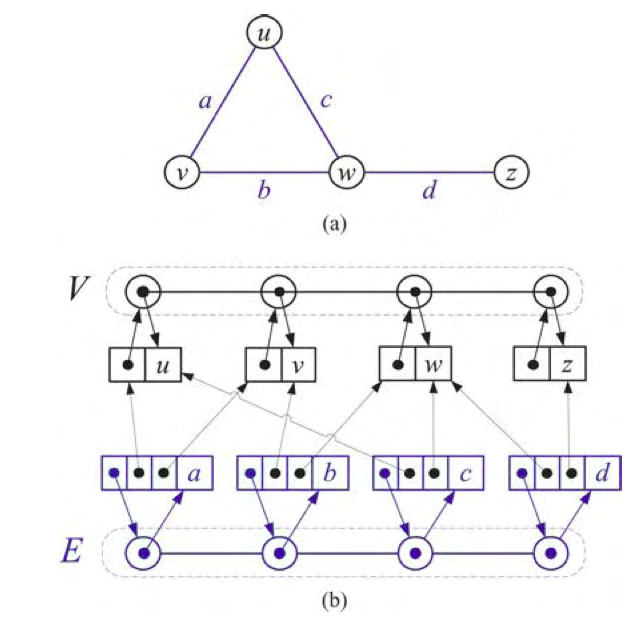
\includegraphics[width=0.8\textwidth]{edgeslist.png}\\
Edge List\\
source: Data Structures and Algorithms in Java Fourth Edition
\end{center}
RemoveEdge est de complexité O(1) puisqu'il s'agit d'une liste doublement chainée, tout comme insertVertex.\\

La réponse dépend bien de la structure de données utilisées pour mémoriser les contenus. Si les edges étaient stockées par vertex, il serait possible d'avoir de bien meilleures performances lors de l'opération removeVertex.\\

Le concept de location aware entry est indispensable pour avoir une complexité O(1) pour la méthode removeEdge.

\paragraph{Question 2 (Grynczel Wojciech) Quelle est la complexité temporelle d’un parcours en largeur d’abord pour un	graphe simple comportant n noeuds lorsque ce graphe est représenté par une matrice d’adjacence ? Justifiez votre réponse.\\}

$ O(n^2) $ 	n = nombre de noeuds\\
Justification: Avec une matrice adjacente on doit vérifier, pour chaque sommet  tous les arêtes sortants possibles.


\paragraph{Question 3}

\paragraph{Question 4}

\paragraph{Question 5 (Bertaux Jérôme) On considère un réseau téléphonique qui peut être vu comme un graphe G dont les sommets représentent des terminaux de commutation et les arcs représentent des lignes de communication entre ces terminaux. Chaque arc est étiqueté par la bande passante de la ligne qu’il représente. La bande passante d’un chemin dans le graphe est la bande passante de son arc de bande passante minimale (autrement dit, le maillon faible !...). On s'intéresse à l’algorithme \textit{MaxBandWidth(G, a, b)} qui, étant donné un réseau, représenté par un graphe G, et deux terminaux a et b, renvoie la bande passante maximale d’un chemin entre a et b. Donnez le pseudo- code de l’algorithme \textit{MaxBandWidth(G, a, b)}. Piste de solution : pensez à une variante d’un algorithme bien connu présenté dans le livre de référence.}

Le principe est qu'il faut parcourir tout le graphe en trouvant l'arc (les lignes de communication entre les terminaux) dont la bande passante est la plus faible. L'algorithme de \textit{MaxBandWidth(G, a, b)} est inspiré de l'algorithme de Dijkstra.\\

Pseudo-code de \textit{MaxBandWidth(G, a, b)}:\\
     Input: un graphe simple G non dirigé dont chacune des arêtes se voit attribuer une capacité maximale (bande passante maximale), ainsi que deux nœuds a,b de G.
	 
     Output: une étiquette D[b], pour chaque nœud b de G, tel que D[b] est la bande passante maximale d’un chemin entre a et b dans G.
      
      Initialize D[a] = 0 et D[b] =  $\infty$ pour chaque noeud b $\neq$ a\\
      Soit Q la file de priorité contenant tous les nœuds de G en prenant les étiquettes D comme étant les clés.
\begin{verbatim}
Algorithm MaxBandWidth(G, a, b):
     while Q is not empty do
          u = Q.removeMin()
          for each edge (u,b) such that b is in Q do
               if D[u] + w(u,b) < D[b] then
                    D[b] = D[u] + w(u,v)
                    Change the key of vertex b in Q to D[b].
     return the label D[b] of each vertex v
\end{verbatim}




\paragraph{Question 6 (Charles Jacquet) Quelle est la complexité temporelle de votre algorithme MaxBandWidth(G, a, b) (décrit à la question 5) ? Précisez notamment les hypothèses éventuelles sur l’implémentation des structures de données utilisées, dans la mesure où ces hypothèses seraient importantes pour justifier la complexité annoncée.}



\end{document}
